\uuid{bR1F}
\niveau{PCSI}
\module{Analyse}
\chapitre{Convergence d'une suite}
\sousChapitre{Suite, monotonie et point fixe}
\duree{30}
\difficulte{1}
\auteur{Antoine Crouzet}
\datecreate{01/12/2024}
\titre{Suites et point fixe I}
\contenu{
\texte{On considère la suite $(u_n)_{n\in\N}$ définie par $u_0=1$ et, pour $n\geq 0$, $u_{n+1}=\dfrac{u_n}{u_n +1}$.}
\question{Soit  $f$ la fonction d\'efinie sur $]-1;+\infty[$ par  : $f(x)=\dfrac{x}{x+1}$. 
 Montrer que si $x\in [0;1]$, alors $f(x)\in [0;1]$.}
\reponse{\begin{align*}
\label{td-10-q1} La fonction $f$ est définie et dérivable sur $]-1;+\infty[$. Pour tout $x>-1$, on a \[ f'(x)=\frac{1(x+1)-x1}{(x+1)^2} = \frac{1}{(x+1)^2} \]
		Pour tout réel $x>1$, $f'(x)>0$. La fonction $f$ est donc strictement croissante sur $]-1;+\infty[$. On obtient le tableau de variations suivant :
\begin{center}	\begin{tikzpicture}
	   \tkzTabInit[lgt = 2, espcl = 5]{$x$ / 1 , $f'(x)$ / 1, Variations de $f$ / 2}{$-1$, $+\infty$}
	   \tkzTabLine{d, +,  }
	   \tkzTabVar{D-/ , +/ }
	   \tkzTabVal{1}{2}{0.3}{$0$}{$0$}
	   \tkzTabVal{1}{2}{0.7}{$1$}{$\frac{1}{2}$}
	\end{tikzpicture}
\end{center}
Par croissance de $f$ sur $]-1;+\infty[$, on constate alors que si $0\leq x\leq 1$, alors \[0=f(0)\leq f(x)\leq f(1)=\frac12 \leq 1.\]
\begin{remarque}
	On dit que l'invervalle $[0;1]$ est \textbf{stable} par $f$.
\end{remarque}
\end{align*}}
\question{Montrer que pour tout $n\geq 0$, $u_n\in[0;1]$.}
\reponse{\begin{align*}
\label{td-10-q2} Soit $P$ la proposition définie pour tout entier naturel $n$ par $P_n$ : ``$u_n\in [0;1]$''. \\
		\textbf{Initialisation} : pour $n=0$, on constate que $u_0=1\in [0;1]$ : $P_0$ est vraie.\\
		\textbf{Hérédité} : supposons la proposition $P_n$ vraie pour un certain entier $n$ fixé. On a alors, par hypothèse de récurrence, $u_n\in [0;1]$. Mais alors, d'après la question \ref{td-10-q1}, $f(u_n)\in [0;1]$, c'est-à-dire $u_{n+1}\in [0;1]$. Ainsi, $P_{n+1}$ est vraie et la proposition est héréditaire.\\
		D'après le principe de récurrence, la proposition $P_n$ est vraie pour tout $n$, et ainsi \[ \forall~n\in \N,\quad u_n\in [0;1] \]
\end{align*}}
\question{\'Etudier le signe de $f(x)-x$ sur $]-1;+\infty[$.}
\reponse{\label{td-10-q3} Soit $x\in ]-1;+\infty[$. On a 
	\begin{align*}
		f(x)-x &= \frac{x}{x+1}- x \\
		&= \frac{x-x(x+1)}{x+1} = \frac{-x^2}{x+1}
	\end{align*}
	Puisque $x\in ]-1;+\infty[$, $x+1>0$ et $-x^2<0$. Ainsi, pour tout $x\in ]-1;+\infty[$, $f(x)-x<0$.}
\question{Montrer que $(u_n)_{n\in\N}$ est d\'ecroissante.}
\reponse{\begin{align*}
\label{td-10-q4} Soit $n\in \N$. D'après la question \ref{td-10-q2}, $u_n\in [0;1]$. On peut donc appliquer la résultat précédent à $x=u_n\in ]-1;+\infty[$ et on obtient $f(u_n)-u_n<0$, c'est-à-dire $u_{n+1}-u_n<0$. Ceci étant valable pour tout entier $n$, on en déduit que la suite $(u_n)$ est (strictement) décroissante.
\end{align*}}
\question{En déduire que  $(u_n)_{n\in\N}$ converge.}
\reponse{\begin{align*}
D'après la question \ref{td-10-q4}, la suite $(u_n)$ est décroissante. Mais d'après la question \ref{td-10-q2}, elle est bornée, et donc minorée (par $0$). D'après le théorème de la limite monotone, on peut donc dire que la suite $(u_n)$ converge.
\end{align*}}
\question{Déterminer la limite de $(u_n)_{n\in\N}$.}
\reponse{\begin{align*}
La suite $(u_n)$ converge. Notons $\ds{\ell=\lim_{n\to+\infty} u_n}$. D'après ce qui précède, $\ell \geq 0$. Mais alors, par somme et quotient de limite
	\[ \lim_{n\to +\infty} \frac{u_n}{u_n+1} = \frac{\ell}{\ell + 1}\] De plus, $\ell$ est également la limite de la suite $(u_{n+1})$. En utilisant la relation de définition et en passant à la limite, on en déduit \[ \ell = \frac{\ell}{\ell+1} \]
	c'est-à-dire $\ell(\ell+1)=\ell$, soit encore $\ell^2=0$, et finalement $\ell=0$.
	\\\textbf{Bilan} : la suite $(u_n)$ converge verss $0$.
\begin{remarque}
	Le raisonnement précédent, qu'on précisera plus tard dans l'année, s'appelle le \textbf{théorème du point fixe} et dit (sous condition sur $f$) que si $u_{n+1}=f(u_n)$ et que la suite $(u_n)$ converge, alors la limite $\ell$ vérifie $\ell=f(\ell)$, c'est-à-dire est un \textbf{point fixe} de $f$.
	\end{remarque}
\end{align*}}
}
